
\section{Extra Numerical Results \label{supp_matt:numericalresults}}

In this section, we present extra numerical results to supplement those in the main text. 

Firstly, we will elaborate on our goals. We aim for two properties that our cost functions should exhibit in order to claim they have outperformed the $\MMD$ training method:
\begin{itemize}
    \item \textit{Speed of Converge:} Both cost functions, $\SD$ and $\SH$ should achieve equal or lower $\TV$ than the $\MMD$ in a \textit{shorter} time period (even accounting for various learning rates).
    \item \textit{Accuracy:} Since the cost functions we employ are in some sense `stronger' than $\MMD$, we want to see them achieve a \textit{smaller} $\TV$ than is possible with the $\MMD$ in an equal or quicker time. %In this somewhat absolute sense, one could claim the training methods are better. 
\end{itemize}

It should be noted that the $\TV$ appears to behave strangely during training, often initially increasing. The reason for this is that it is not be minimised \textit{directly}, only through auxiliary cost functions. As such, we would not expect to see a monotonically decreasing curve. It is also clear that it would not be possible to compute $\TV$ in general as the number of qubits scales, but it is possible to do so to benchmark the small examples we use here. 


Firstly, we revisit the Quantum (\eqref{quantumkernel}) vs.\@ Gaussian  (\eqref{gaussiankernel}) kernels of the main text with the corresponding example for two qubits in \figref{fig:QvGkernel2}. These results corroborate those seen in the main text for four qubits, that $\kappa_Q$ is both suitable for training the $\IBM$, and seems to converge faster when used in the $\MMD$ with all other parameters being identical. This is indicated in \figref{subfig:tv_2_qubits_mmd_gaussian_v_quantum} and \figref{subfig:tv_4_qubits_mmd_gaussian_v_quantum}. However, the computation of this kernel is likely to not be feasible for near term quantum devices, but does reinforce the potential of quantum kernels first explored in refs. \citeS{havlicek_supervised_2019, schuld_quantum_2019}. 

Again, the data was taken during 5 independent runs in each case, with averages and errors computed over the runs. This behaviour is apparent even for a range of learning rates. In the two qubit case, there is not a major difference between the two, but the discrepancy becomes more apparent as the number of qubits increases. This could be an indicator of the quantum kernel's extra expressive power and ability to capture finer details of the distribution, as in the four qubit case it can actually achieve a \textit{lower} $\TV$ than the Gaussian kernel, used in \citeS{liu_differentiable_2018}. Of course, this quantum kernel may not outperform all other kernels, or even different choices of the bandwith parameters in \eqref{gaussiankernel}, but it is encouraging that such results were observed on a randomly selected dataset. Whether or not this performance is due to some fundamental `quantum' reason, or simply that the kernel is more complicated, requires further study. However, the latter seems unlikely since the dataset is completely classical.

\begin{figure}
    \centering
    \begin{subfigure}[t]{0.29\textwidth}
    \centering
        % \includegraphics[width=\textwidth, height = 0.9\textwidth]{images/TV_2_qubits_mmd_kernel_comp_lr_Average_samples_500_batch_250.pdf}
        \begin{tikzpicture}
  \node (img)  {\includegraphics[width=\textwidth, height = 0.8\textwidth]{images/FIG_S1a_TV_2_qubits_mmd_kernel_comp_lr_Average_samples_500_batch_250.pdf}};
  \node[below=of img, node distance=0cm, yshift=1.35cm,font=\color{black}] {epochs};
  \node[left=of img, node distance=0cm, rotate=90, anchor=center,yshift=-0.95cm,font=\color{black}] {$\TV$};
\end{tikzpicture}
        \caption{}
        \label{subfig:tv_2_qubits_mmd_gaussian_v_quantum}
    \end{subfigure}
    ~ \centering
    \begin{subfigure}[t]{0.29\textwidth}
    \centering
        % \includegraphics[width=\textwidth, height = 0.9\textwidth]{images/probs_2_qubits_mmd_kernel_comp_lr_0_08_AVG_samples_500_batch_250.pdf}
        \begin{tikzpicture}
  \node (img)  {\includegraphics[width=\textwidth, height = 0.8\textwidth]{images/FIG_S1b_probs_2_qubits_mmd_kernel_comp_lr_0_08_AVG_samples_500_batch_250.pdf}};
  \node[below=of img, node distance=0cm, yshift=1.35cm,font=\color{black}] {outcomes};
  \node[left=of img, node distance=0cm, rotate=90, anchor=center,yshift=-0.95cm,font=\color{black}] {probability};
\end{tikzpicture}
        \caption{}
        \label{subfig:probs_2_qubits_mmd_gaussian_v_quantum}
    \end{subfigure}
    ~ \centering
    \begin{subfigure}[t]{0.29\textwidth}
    \centering
        % \includegraphics[width=\textwidth, height = 0.9\textwidth]{images/MMD_2_qubits_mmd_kernel_comp_Average_samples_500_batch_250.pdf}
        \begin{tikzpicture}
  \node (img)  {\includegraphics[width=\textwidth, height = 0.8\textwidth]{images/FIG_S1c_MMD_2_qubits_mmd_kernel_comp_Average_samples_500_batch_250.pdf}};
  \node[below=of img, node distance=0cm, yshift=1.35cm,font=\color{black}] {epochs};
  \node[left=of img, node distance=0cm, rotate=90, anchor=center,yshift=-0.95cm,font=\color{black}] {$\MMD$ loss $\mathcal{L}_{\MMD}$};
\end{tikzpicture}
        \caption{}
        \label{subfig:mmd_kernel_comp_2_qubits}
    \end{subfigure}
    \caption{Performance of quantum $\kappa_Q$ [\crule[red]{0.2cm}{0.2cm}] vs. Gaussian kernel,  $\kappa_G$ [\crule[blue]{0.2cm}{0.2cm}] (with $\eta_{\mathsf{init}} = 0.1$) for 2 qubits. To train, we sample from the $\IBM$ and the data $500$ times and use a minibatch size of $250$. One epoch is one complete update of all parameters according to gradient descent. Error bars represent maximum, minimum and mean values achieved over 5 independent training runs, with the same initial conditions on the same data samples. (a) $\TV$ Difference achieved with both kernel methods during training. With the quantum kernel, a lower value of $\TV$ can be achieved than with a Gaussian kernel. Increasing the learning rate speeds up convergence, but still cannot achieved the same minimum $\TV$ (b) Final learned probabilities with $\eta_{\mathsf{init}} = 0.1$ using the Adam optimiser. (c) $\MMD$ computed using $400$ samples as training points, $100$ as test points, independent of the training data. $\MMD$ is seen to converge faster with the quantum kernel, although it appears to have a higher generalisation error.}
    \label{fig:QvGkernel2}
\end{figure}


Next, \figref{fig:MMDvSinkvStein4} illustrate the differences between using the $\MMD$ cost function and either the Sinkhorn Divergence or the Stein discrepancy for three qubits, to supplement \figref{fig:MMDvSinkvStein3} in the main text. We found that with the exception of the two qubit case, both the Stein discrepancy and the Sinkhorn divergence are able to learn with a higher \textit{speed of convergence}, and \textit{accuracy} as shown in \figref{subfig:tv_4_qubits_mmd_v_sinkhorn}, reinforcing \figref{subfig:tv_3_qubits_mmd_v_sinkhorn} in the main text. It should be noted that the results for the Sinkhorn training were highly dependent on the value of the regularisation, as expected. Also, simply because the Sinkhorn achieved better results on one particular data set, does not imply that it would do so over most. 

In the case of the Stein discrepancy, we run the training algorithm only for 125 epochs. The reason for this is twofold. Firstly, when training using the `exact' Stein score (i.e.\@ with oracle access to the data probabilities $\pi$) the convergence was so fast that the model would tend to jump out of its attained minimum after a certain period of time. Hence we employed a form of early stopping, as indicated in \figref{subfig:tv_4_qubits_mmd_v_sinkhorn}. Secondly, for the case of the `Spectral' Score method, (\figref{subfig:tv_3_qubits_mmd_v_sinkhorn} and \figref{subfig:tv_4_qubits_mmd_v_sinkhorn}) we used much less samples than with the previous methods. This is due to the (classical) computational cost of computing the Score using this method in our naive implementation. We also took the best run of the Stein training algorithm, rather than an average in the other cases. This was due to the low sample numbers, which lead to a high deviation in the training path taken, so we removed it in order to not obscure the other results. For computing the Spectral Score, we used 3 and 6 Nystr{\"o}m eigenvectors for 3 and 4 qubits respectively, for details see \appref{supp_matt:steinscoremethod}. 

Finally, one may comment on the fact that we allowed the Stein Discrepancy to use the exact probabilities of the data, $\pi$, and this constitutes an unfair advantage against the $\MMD$. In fact, the high number of samples we used ensured that the approximate data distributions that the $\MMD$ received was in fact very close to the exact data, and we found no major improvement for training with the $\MMD$ by allowing oracle data access, i.e.\@ the exact probabilities, $\pi$, reinforcing the fundamental weakness of the $\MMD$ that is discussed above.  
\begin{figure*}[ht]
    \centering
    %  \begin{subfigure}[t]{0.3\textwidth}
    %  \centering
    %     \includegraphics[width=0.8\textwidth]{images/3qubit_fullConnect.pdf}
    %     \vskip 2pt
    %     \caption{}
    %     \label{subfig:3_qubit_topology}
    % \end{subfigure}
%     \begin{subfigure}[t]{0.3\textwidth}
%         % \includegraphics[width=\textwidth, height = 0.8\textwidth]{images/TV_3_qubits_mmd_stein_sinkhorn_3_evecs_eps_0_08_.pdf}
% \begin{tikzpicture}
%   \node (img)  {\includegraphics[width=\textwidth, height = 0.8\textwidth]{images/TV_3_qubits_mmd_stein_sinkhorn_3_evecs_eps_0_08_.pdf}};
%   \node[below=of img, node distance=0cm, yshift=1.35cm,font=\color{black}] {epochs};
%   \node[left=of img, node distance=0cm, rotate=90, anchor=center,yshift=-0.95cm,font=\color{black}] {$\TV$};
% \end{tikzpicture}
%         \caption{}
%         \label{subfig:tv_3_qubits_mmd_v_sinkhorn}
%     \end{subfigure}
%     ~ %add desired spacing between images, e. g. ~, \quad, \qquad, \hfill etc. 
%       %(or a blank line to force the subfigure onto a new line)
%     \begin{subfigure}[t]{0.3\textwidth}
%         % \includegraphics[width=\textwidth, height = 0.8\textwidth]{images/Probs_3_qubits_mmd_stein_sinkhorn_3_evecs_eps_0_08_.pdf}
%           \begin{tikzpicture}
%   \node (img)  {\includegraphics[width=\textwidth, height = 0.8\textwidth]{images/Probs_3_qubits_mmd_stein_sinkhorn_3_evecs_eps_0_08_.pdf}};
%   \node[below=of img, node distance=0cm, yshift=1.35cm,font=\color{black}] {outcomes};
%   \node[left=of img, node distance=0cm, rotate=90, anchor=center,yshift=-0.95cm,font=\color{black}] {probability};
% \end{tikzpicture}
%         \caption{}
%         \label{subfig:probs_3_qubits_mmd_mmd_v_sinkhorn}
%     \end{subfigure}
    ~ %add desired spacing between images, e. g. ~, \quad, \qquad, \hfill etc. 
    %(or a blank line to force the subfigure onto a new line)
    \begin{subfigure}[t]{0.3\textwidth}
        % \includegraphics[width=\textwidth, height = 0.8\textwidth]{images/SINK_3_qubits_mmd_stein_sinkhorn_3_evecs_eps_0_08.pdf}
          \begin{tikzpicture}
  \node (img)  {\includegraphics[width=\textwidth, height = 0.8\textwidth]{images/FIG_S2a_SINK_3_qubits_mmd_stein_sinkhorn_3_evecs_eps_0_08.pdf}};
  \node[below=of img, node distance=0cm, yshift=1.35cm,font=\color{black}] {epochs};
  \node[left=of img, node distance=0cm, rotate=90, anchor=center,yshift=-0.95cm,font=\color{black}] {Sinkhorn loss $\mathcal{L}_{\SH}$};
\end{tikzpicture}
        \caption{}
        \label{subfig:sinkhorn_3_qubits}
    \end{subfigure}
    ~
    \begin{subfigure}[t]{0.3\textwidth}
        % \includegraphics[width=\textwidth, height = 0.8\textwidth]{images/MMD_3_qubits_mmd_stein_sinkhorn_3_evecs_eps_0_08.pdf}
        \begin{tikzpicture}
  \node (img)  {\includegraphics[width=\textwidth, height = 0.8\textwidth]{images/FIG_S2b_MMD_3_qubits_mmd_stein_sinkhorn_3_evecs_eps_0_08.pdf}};
  \node[below=of img, node distance=0cm, yshift=1.35cm,font=\color{black}] {epochs};
  \node[left=of img, node distance=0cm, rotate=90, anchor=center,yshift=-0.95cm,font=\color{black}] {MMD loss $\mathcal{L}_{\MMD}$};
\end{tikzpicture}
        \caption{}
        \label{subfig:mmd_3_qubits}
    \end{subfigure}
    ~
    \begin{subfigure}[t]{0.3\textwidth}
        % \includegraphics[width=\textwidth, height = 0.8\textwidth]{images/STEIN_3_qubits_mmd_stein_sinkhorn_3_evecs_eps_0_08.pdf}
\begin{tikzpicture}
  \node (img)  {\includegraphics[width=\textwidth, height = 0.8\textwidth]{images/FIG_S2c_STEIN_3_qubits_mmd_stein_sinkhorn_3_evecs_eps_0_08.pdf}};
  \node[below=of img, node distance=0cm, yshift=1.35cm,font=\color{black}] {epochs};
  \node[left=of img, node distance=0cm, rotate=90, anchor=center,yshift=-0.95cm,font=\color{black}] {Stein loss $\mathcal{L}_{\SD}$};
\end{tikzpicture}
        \caption{}
        \label{subfig:stein_3_qubits}
    \end{subfigure}
    \caption{$\MMD$ [\crule[cyan]{0.2cm}{0.2cm}, \crule[yellow]{0.2cm}{0.2cm}, \crule[ForestGreen]{0.2cm}{0.2cm}] vs.\@ Sinkhorn [\crule[blue]{0.2cm}{0.2cm}] and Stein training with Exact score function [\crule[red]{0.2cm}{0.2cm}] and Spectral score method [\crule[magenta]{0.2cm}{0.2cm}] for 3 qubits with fully connected topology, Rigetti {\fontfamily{cmtt}\selectfont 3q-qvm}, \protect\begin{tikzpicture}[transform canvas={scale=0.09}]
%% vertices
\draw[fill=gray] (0,0) circle (20pt);
\draw[fill=gray] (4,0) circle (20pt);
\draw[fill=gray] (2,3) circle (20pt);
%% vertex labels
%%% edges
\draw[gray, thick] (0,0) -- (4,0) -- (0,0) -- (2,3) -- (4,0) -- (2,3);
\end{tikzpicture}
\ \ \ , trained on the data, \eqref{toydatadistribution}. 500 data points are used for training, with 400 used as a training set, and 100 used as a test set for all except the Stein discrepancy using the spectral score, which used only 40 samples. Plots show mean, maximum and minimum values achieved over 5 independent training runs on the same dataset. (a) $\mathcal{L}^{0.08}_{\SH}$   using 500 samples and a batch size of 250. (b) $\mathcal{L}_{\MMD}$ using 500 samples and a batch size of 250, with three different initial learning rates. (c) $\mathcal{L}_{\SD}$ using 500 samples and a batch size of 250 for Exact score, and 40 samples and batch size of 20 for the Spectral score. Corresponds to \figref{fig:MMDvSinkvStein3} in main text.}\label{fig:MMDvSinkvStein3_supp}
\end{figure*}

\begin{figure}
    \centering
%     \begin{subfigure}[t]{0.38\textwidth}
%      \centering
%         % \includegraphics[width=0.7\textwidth]{images/4qubit_fullConnect.pdf}
%          \begin{tikzpicture}
%   \node (img)  {\includegraphics[width=0.7\textwidth]{images/4qubit_fullConnect.pdf}};
%   \node[below=of img, node distance=0cm, yshift=1.35cm,font=\color{black}] {};
%   \node[left=of img, node distance=0cm, rotate=90, anchor=center,yshift=-0.95cm,font=\color{black}] {};
%   \end{tikzpicture}
%         \vskip 5pt
%         \caption{}\label{subfig:4_qubit_topology}
%     \end{subfigure}
    ~
    \begin{subfigure}[t]{0.35\textwidth}
    \centering
        % \includegraphics[width=\textwidth, height = 0.8\textwidth]{images/TV_4_qubits_mmd_stein_sinkhorn_6_evecs_eps_0_08_.pdf}
        \begin{tikzpicture}
  \node (img)  {\includegraphics[width=\textwidth, height = 0.8\textwidth]{images/FIG_S3a_TV_4_qubits_mmd_stein_sinkhorn_6_evecs_eps_0_08.pdf}};
  \node[below=of img, node distance=0cm, yshift=1.35cm,font=\color{black}] {epochs};
  \node[left=of img, node distance=0cm, rotate=90, anchor=center,yshift=-0.95cm,font=\color{black}] {$\TV$};
\end{tikzpicture}
        \caption{}
        \label{subfig:tv_4_qubits_mmd_v_sinkhorn}
    \end{subfigure}
    ~
    \begin{subfigure}[t]{0.35\textwidth}
    \centering
        % \includegraphics[width=\textwidth, height = 0.8\textwidth]{images/PROBS_4_qubits_mmd_stein_sinkhorn_6_evecs_eps_0_1_.pdf}
        \begin{tikzpicture}
  \node (img)  {\includegraphics[width=\textwidth, height = 0.8\textwidth]{images/FIG_S3b_PROBS_4_qubits_mmd_stein_sinkhorn_6_evecs_eps_0_08.pdf}};
  \node[below=of img, node distance=0cm, yshift=1.35cm,font=\color{black}] {outcomes};
  \node[left=of img, node distance=0cm, rotate=90, anchor=center,yshift=-0.95cm,font=\color{black}] {probability};
\end{tikzpicture}
        \caption{}
        \label{subfig:probs_4_qubits_mmd_mmd_v_sinkhorn}
    \end{subfigure}
    ~
    \begin{subfigure}[t]{0.35\textwidth}
    \centering
        % \includegraphics[width=\textwidth, height = 0.8\textwidth]{images/SINK_4_qubits_mmd_stein_sinkhorn_6_evecs_eps_0_1.pdf}
        \begin{tikzpicture}
  \node (img)  {\includegraphics[width=\textwidth, height = 0.8\textwidth]{images/FIG_S3c_SINK_4_qubits_mmd_stein_sinkhorn_6_evecs_eps_0_08.pdf}};
  \node[below=of img, node distance=0cm, yshift=1.35cm,font=\color{black}] {epochs};
  \node[left=of img, node distance=0cm, rotate=90, anchor=center,yshift=-0.95cm,font=\color{black}] {Sinkhorn loss $\mathcal{L}_{\SH}$};
\end{tikzpicture}
        \caption{}
        \label{subfig:sinkhorn_4_qubits}
    \end{subfigure}
    ~
    \begin{subfigure}[t]{0.35\textwidth}
    \centering
        % \includegraphics[width=0.9\textwidth, height = 0.8\textwidth]{images/MMD_4_qubits_mmd_stein_sinkhorn_3_evecs_eps_0_1.pdf}
        \begin{tikzpicture}
  \node (img)  {\includegraphics[width=\textwidth, height = 0.8\textwidth]{images/FIG_S3d_MMD_4_qubits_mmd_stein_sinkhorn_6_evecs_eps_0_08.pdf}};
  \node[below=of img, node distance=0cm, yshift=1.35cm,font=\color{black}] {epochs};
  \node[left=of img, node distance=0cm, rotate=90, anchor=center,yshift=-0.95cm,font=\color{black}] {$\MMD$ loss $\mathcal{L}_{\MMD}$};
\end{tikzpicture}
        \caption{}
        \label{subfig:mmd_4_qubits}
    \end{subfigure}
    ~
    \begin{subfigure}[t]{0.35\textwidth}
    \centering
        % \includegraphics[width=0.9\textwidth, height = 0.8\textwidth]{images/STEIN_4_qubits_mmd_stein_sinkhorn_6_evecs_eps_0_08_.pdf}
        \begin{tikzpicture}
  \node (img)  {\includegraphics[width=\textwidth, height = 0.8\textwidth]{images/FIG_S3e_STEIN_4_qubits_mmd_stein_sinkhorn_6_evecs_eps_0_08.pdf}};
  \node[below=of img, node distance=0cm, yshift=1.35cm,font=\color{black}] {epochs};
  \node[left=of img, node distance=0cm, rotate=90, anchor=center,yshift=-0.95cm,font=\color{black}] {Stein loss $\mathcal{L}_{\SD}$};
\end{tikzpicture}
        \caption{}
        \label{subfig:stein_4_qubits}
    \end{subfigure}
    \caption{$\MMD$ [\crule[cyan]{0.2cm}{0.2cm}, \crule[yellow]{0.2cm}{0.2cm}, \crule[ForestGreen]{0.2cm}{0.2cm}] vs.\@ Sinkhorn [\crule[blue]{0.2cm}{0.2cm}]  with regularisation parameter $\epsilon = 0.08$ and Stein training with Spectral score method [\crule[magenta]{0.2cm}{0.2cm}] using 6 eigenvectors for 4 qubits. We use qubit topology in fully connected graph for four qubits, i.e.\@ Rigetti {\fontfamily{cmtt}\selectfont 4q-qvm},  \protect\begin{tikzpicture}[transform canvas={scale=0.08}]
%% vertices
\draw[fill=gray] (0,0) circle (20pt);
\draw[fill=gray] (4,0) circle (20pt);
\draw[fill=gray] (0,4) circle (20pt);
\draw[fill=gray] (4,4) circle (20pt);
%% vertex labels
%%% edges
\draw[gray, thick] (0,0) -- (4,0) -- (4,4) -- (0,4) -- (0,0) -- (4,4) -- (4,0) -- (0,4) ;
\end{tikzpicture}\ \ \ . Plots show mean, maximum and minimum values over 5 independent training runs on the same dataset. (a) $\TV$ Difference between training methods. Both Sinkhorn divergence and Stein discrepancy can achieve lower $\TV$ values than the $\MMD$. (b) Final learned probabilities of target data, \eqref{toydatadistribution} [\crule[black]{0.2cm}{0.2cm}]. (c) $\mathcal{L}^{0.08}_{\SH}$ using 500 samples and a batch size of 250. 400 samples used as a training set, 100 for the test set. Trained using Hamming optimal transport cost function (d) $\mathcal{L}_{\MMD}$ using 500 samples and a batch size of 250, with three different initial learning rates. (e) $\mathcal{L}_{\SD}$ using 30 Samples and batch size of 20 for the Spectral score using a learning rate $\eta_{init}=0.08$. 24 samples used as training data, 6 samples used for test set.}\label{fig:MMDvSinkvStein4}
\end{figure}
% \restoregeometry

We also performed experiments on the 16 Qubit QPU of Rigetti, {\fontfamily{cmtt}\selectfont Aspen}, as seen in \figref{fig:MMDvSinkvStein3_real} and \figref{fig:MMDvSink4_real} in the main text, to determine the performance of the training on real quantum hardware. We used two sublattices for 3 and 4 qubits respectively, the {\fontfamily{cmtt}\selectfont Aspen-4-3Q-A} and {\fontfamily{cmtt}\selectfont Aspen-4-4Q-A}, and their respective {\fontfamily{cmtt}\selectfont qvm} versions. As before we ran 5 independent runs of the training procedure from the same initial condition, and took averages over the run. We restricted to the native connectivity of the chip, as seen in \figref{subfig:3_qubit_topology_aspen_4_3q_a}, and used the available qubits in the {\fontfamily{cmtt}\selectfont Aspen-4-3Q-A} chip, $(10, 11, 17)$, with no direct connection between qubits $11$ and $17$, as illustrated. Taking this into account, we did not enforce a fully connected topology, and any of the real on-chip experiments, since this would have resulted in the compiler implementing SWAP gates. This is one reason why the models trained reasonably well on the hardware, with the fact that the two qubit gates in our $\IBM$ are close to being native to the Rigetti chip (where CZ gates are the native entangling links) also providing an advantage.

\figref{subfig:tv_3_qubits_mmd_v_sinkhorn_real} compares training using the $\MMD$ with a Gaussian kernel and the Sinkhorn Divergence, benchmarked relative to $\TV$ as with the previous numerical results. As expected, the QPU noise leads to a higher variance between training runs, but the large number of samples taken $(500)$ still permits the model to learn quickly. This reproduces the behaviour seen in \figref{subfig:tv_4_qubits_mmd_v_sinkhorn_real} in the main text. In both examples, it can been observed that the Sinkhorn cost function enabled faster and more accurate training, which becomes more evident as the number of qubits increases. It was also necessary to use quite an aggressive learning rate for four qubits while training with the $\MMD$ over $\SH$, $0.15 \text{ vs. } 0.1$, in order to get the model to train \textit{at all} within the given number of epochs. 


\begin{figure}
    \centering
    \begin{subfigure}[t]{0.38\textwidth}
        % \includegraphics[width=\textwidth, height = 0.8\textwidth]{images/TV_3_qubits_ASPEN-4-3Q-A_mmd_sinkhorn_evecs_eps_0_08_.pdf}
                       \begin{tikzpicture}
  \node (img)  {\includegraphics[width=\textwidth, height = 0.8\textwidth]{images/FIG_S4a_TV_3_qubits_ASPEN-4-3Q-A_mmd_sinkhorn_evecs_eps_0_08_.pdf}};
  \node[below=of img, node distance=0cm, yshift=1.35cm,font=\color{black}] {epochs};
  \node[left=of img, node distance=0cm, rotate=90, anchor=center,yshift=-0.95cm,font=\color{black}] {$\TV$};
\end{tikzpicture}
        \caption{}
        \label{subfig:tv_3_qubits_mmd_v_sinkhorn_real}
    \end{subfigure}
    ~
    \begin{subfigure}[t]{0.38\textwidth}
        % \includegraphics[width=\textwidth, height = 0.8\textwidth]{images/PROBS_3_qubits_ASPEN-4-3Q-A_mmd_two_runs_sinkhorn_evecs_eps_0_08_.pdf}
                       \begin{tikzpicture}
  \node (img)  {\includegraphics[width=\textwidth, height = 0.8\textwidth]{images/FIG_S4b_PROBS_3_qubits_ASPEN-4-3Q-A_mmd_sinkhorn_eps_0_08.pdf}};
  \node[below=of img, node distance=0cm, yshift=1.35cm,font=\color{black}] {outcomes};
  \node[left=of img, node distance=0cm, rotate=90, anchor=center,yshift=-0.95cm,font=\color{black}] {probability};
\end{tikzpicture}
        \caption{}
        \label{subfig:probs_3_qubits_mmd_v_sinkhorn_real}
    \end{subfigure}
    ~
    \begin{subfigure}[t]{0.38\textwidth}
        % \includegraphics[width=\textwidth, height = 0.8\textwidth]{images/SINK_3_qubits_ASPEN-4-3Q-A_mmd_sinkhorn_evecs_eps_0_08_.pdf}
                       \begin{tikzpicture}
  \node (img)  {\includegraphics[width=\textwidth, height = 0.8\textwidth]{images/FIG_S4c_SINK_3_qubits_ASPEN-4-3Q-A_mmd_sinkhorn_eps_0_1_lr_0_08.pdf}};
  \node[below=of img, node distance=0cm, yshift=1.35cm,font=\color{black}] {epochs};
  \node[left=of img, node distance=0cm, rotate=90, anchor=center,yshift=-0.95cm,font=\color{black}] {Sinkhorn loss $\mathcal{L}_{\SH}$};
\end{tikzpicture}
        \caption{}
        \label{subfig:sinkhorn_3_qubits_real0_1}
    \end{subfigure}
    ~
     \begin{subfigure}[t]{0.38\textwidth}
        % \includegraphics[width=\textwidth, height = 0.8\textwidth]{images/MMD_3_qubits_ASPEN-4-3Q-A_mmd_sinkhorn_evecs_eps_0_08_.pdf}
    \begin{tikzpicture}
  \node (img)  {\includegraphics[width=\textwidth, height = 0.8\textwidth]{images/FIG_S4d_MMD_3_qubits_ASPEN-4-3Q-A_mmd_sinkhorn_eps_0_08.pdf}};
  \node[below=of img, node distance=0cm, yshift=1.35cm,font=\color{black}] {epochs};
  \node[left=of img, node distance=0cm, rotate=90, anchor=center,yshift=-0.95cm,font=\color{black}] {$\MMD$ loss $\mathcal{L}_{\MMD}$};
\end{tikzpicture}
        \caption{ }
        \label{subfig:mmd_3_qubits_real}
    \end{subfigure}
    ~
     \begin{subfigure}[t]{0.31\textwidth}
     \centering
        \includegraphics[width=0.9\textwidth]{images/FIG_S4e_3qubit_Aspen_4_3Q_A.pdf}
        \vskip 5pt
        \caption{}
        \label{subfig:3_qubit_topology_aspen_4_3q_a}
    \end{subfigure}
    \caption{$\MMD$ vs.\@ Sinkhorn for 3 qubits comparing performance on the real QPU ({\fontfamily{cmtt}\selectfont Aspen-4-3Q-A}) vs.\@ simulated behaviour on QVM ({\fontfamily{cmtt}\selectfont Aspen-4-3Q-A-qvm}) using 500 samples and a batch size of 250. Sinkhorn divergence training outperforms the $\MMD$ both in simulator, and on real hardware relative to total variation. (a) $\TV$ Difference between $\MMD$ [\crule[ForestGreen]{0.2cm}{0.2cm}], and Sinkhorn [\crule[blue]{0.2cm}{0.2cm}] with regularisation parameter $\epsilon = 0.1$ on QVM vs QPU. (b) Final learned probabilities of target data [\crule[black]{0.2cm}{0.2cm}] using $\MMD$ [\crule[ForestGreen]{0.2cm}{0.2cm}] LR $\eta_{\mathsf{init}} = 0.1$ and Sinkhorn [\crule[blue]{0.2cm}{0.2cm}] with $\epsilon = 0.1, \eta_{\mathsf{init}} = 0.08$. (c) $\mathcal{L}^{0.1}_{\SH}$ for 3 qubits trained on the data \eqref{toydatadistribution} on QVM  [\crule[blue]{0.2cm}{0.2cm}] vs.\@ QPU  [\crule[cyan]{0.2cm}{0.2cm}]. (e) $\mathcal{L}_{\MMD}$ for 3 qubits trained on the data \eqref{toydatadistribution} on QVM  [\crule[ForestGreen]{0.2cm}{0.2cm}] vs.\@ QPU  [\crule[cyan]{0.2cm}{0.2cm}]. (f) Qubit `line' topology in Rigetti {\fontfamily{cmtt}\selectfont Aspen-4-3Q-A} chip, using qubits, $(10, 11, 17)$. }\label{fig:MMDvSinkvStein3_real}
\end{figure}

Finally, \figref{fig:autocompilationthreequbits} illustrates the compilation procedure discussed in the main text for three qubits, on the {\fontfamily{cmtt}\selectfont 3q-qvm}. The results are similar to that of the two qubit example; the model is not able to learn \textit{the same} parameters as the target data, but it is able to mimic the output distribution.


\begin{figure}
\centering
\begin{subfigure}[t]{0.45\textwidth}
    \centering
    \includegraphics[width=0.4\textwidth, height = 0.9\textwidth]{images/FIG_S5a_circuit_init_three_qubits_vertical_compressed.pdf}
    \caption{}\label{subfig:auto_comp_3_params}
\end{subfigure}
\begin{subfigure}[t]{0.45\textwidth}
\centering
        % \includegraphics[width=\textwidth, height = 0.9\textwidth]{images/compilation_probs_3_qubits_qaoa_to_IQP_sinkhorn_eps_0_1_lr_0_05_AVERAGE.pdf}
               \begin{tikzpicture}
  \node (img)  {\includegraphics[width=\textwidth, height = 0.8\textwidth]{images/FIG_S5b_compilation_probs_3_qubits_qaoa_to_IQP_sinkhorn_eps_0_1_lr_0_05_AVERAGE_compressed.pdf}};
  \node[below=of img, node distance=0cm, yshift=1.35cm,font=\color{black}] {outcomes};
  \node[left=of img, node distance=0cm, rotate=90, anchor=center,yshift=-0.95cm,font=\color{black}] {probability};
\end{tikzpicture}
    \caption{}
    \label{subfig:auto_comp_final_probs_3}
\end{subfigure}
\begin{subfigure}[t]{0.45\textwidth}
\centering
        % \includegraphics[width=\textwidth, height = 0.9\textwidth]{images/compilation_TV_3_qubits_qaoa_to_IQP_sinkhorn_eps_0_1_lr_0_05_AVERAGE.pdf}
               \begin{tikzpicture}
  \node (img)  {\includegraphics[width=0.9\textwidth, height = 0.8\textwidth]{images/FIG_S5c_compilation_TV_3_qubits_qaoa_to_IQP_sinkhorn_eps_0_1_lr_0_05_AVERAGE_compressed.pdf}};
  \node[below=of img, node distance=0cm, yshift=1.35cm,font=\color{black}] {epochs};
  \node[left=of img, node distance=0cm, rotate=90, anchor=center,yshift=-0.95cm,font=\color{black}] {$\TV$};
\end{tikzpicture}
    \caption{}
    \label{subfig:auto_comp_TV_3}
\end{subfigure}
\begin{subfigure}[t]{0.45\textwidth}
\centering
        % \includegraphics[width=\textwidth, height = 0.9\textwidth]{images/compilation_SINK_3_qubits_qaoa_to_IQP_sinkhorn_eps_0_1_lr_0_05_AVERAGE.pdf}
               \begin{tikzpicture}
  \node (img)  {\includegraphics[width=\textwidth, height = 0.8\textwidth]{images/FIG_S5d_compilation_SINK_3_qubits_qaoa_to_IQP_sinkhorn_eps_0_1_lr_0_05_AVERAGE_compressed.pdf}};
  \node[below=of img, node distance=0cm, yshift=1.35cm,font=\color{black}] {epochs};
  \node[left=of img, node distance=0cm, rotate=90, anchor=center,yshift=-0.95cm,font=\color{black}] {Sinkhorn loss $\mathcal{L}_{\SH}$};
\end{tikzpicture}
    \caption{}
    \label{subfig:auto_comp_sink_3}
\end{subfigure}
\caption{Automatic Compilation of $\IQP$ circuit to a $p = 1 \QAOA$ circuit with three qubits with $\mathcal{L}_{\SH}^\epsilon$ with $\epsilon = 0.1$ A learning rate of $\eta_{init} = 0.05$ was used in the Adam optimiser. $\IBM$ circuit is able to mimic the target distribution well, even though actual achieved parameter values, and circuit families are different. Error bars represent mean, maximum and minimum values achieved over 5 independent training runs on the same data set. (a)  Initial [\crule[cyan]{0.2cm}{0.2cm}] and trained [\crule[Lavender]{0.2cm}{0.2cm}] $\QAOA$ circuit parameters for three qubits. Target $\IQP$ circuit parameters [\crule[green]{0.2cm}{0.2cm}]. (b) Final learned probabilities of $\IBM$ ($\QAOA$) [\crule[blue]{0.2cm}{0.2cm}] circuit versus `data' probabilities ($\IQP$) [\crule[black]{0.2cm}{0.2cm}]. (c) Total Variation Distance during training. (d) Sinkhorn divergence for  400 training samples, 100 test samples, using a Hamming optimal transport cost.}\label{fig:autocompilationthreequbits}
\end{figure}
